\section{Mixer}
\label{sec:mixer}

\subsection{Overview}
\label{sec:mixer-overview}

A mixer modulates the original RF transmission signal with the two amplified RF reception signals to
produce IF signals that encode the distance and incident angle to the remote object (see discussion
in \cref{sec:distance}).

\subsection{5400BL15B050E RF Balun}
\label{sec:5400bl15b050e}

\subsubsection{Description}
\label{sec:5400bl15b050e-description}

The 5400BL15B050E is a balun that supports frequencies of $4.9 - 5.9 \si{GHz}$. It is suggested by
the \hyperref[sec:adl5802]{mixer} datasheet for downconversion from RF to IF\@.

\subsection{ADL5802 Mixer}
\label{sec:adl5802}

\subsubsection{Description}
\label{sec:adl5802-description}

The ADL5802 incorporates two Gilbert cells that allow modulating a local oscillator signal with two
separate RF signals for upconversion or downconversion. It's used here for downconversion to
IF\@. The mixer supports input frequencies of $100 \si{MHz} - 6 \si{GHz}$ and output frequencies of
about $30 \si{kHz} - 600 \si{MHz}$. This fits our requirements which have input frequencies staying
below $5.9 \si{GHz}$ and output frequencies on the order of several hundred kHz.

\subsubsection{Pinout}
\label{sec:adl5802-pinout}



\subsubsection{Component Selection}
\label{sec:adl5802-component-selection}

The input baluns and $3 \si{pF}$ capacitors are specified by the datasheet for the $5.3 - 5.9
\si{GHz}$ frequency we are using. The input interface is shown in
Fig.~\ref{fig:adl5802-input-interface}, which is taken directly from the datasheet. Notice that the
LO positive balanced signal should be connected to LOIN and vice versa.

\begin{figure}[h]
        \centering
        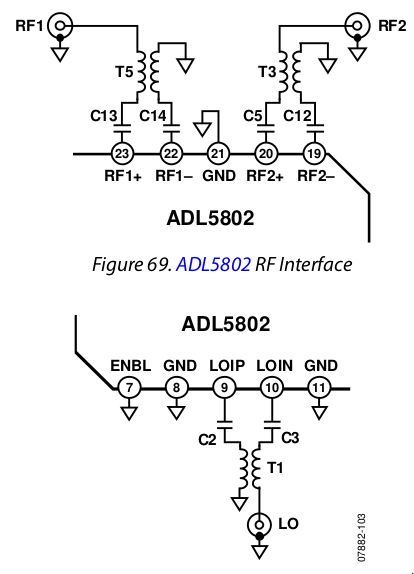
\includegraphics[width=0.3\textwidth]{data/adl5802-input-interface}
        \caption{ADL5802 input interface.}
        \label{fig:adl5802-input-interface}
\end{figure}

\subsubsection{PCB Layout}
\label{sec:adl5802-pcb-layout}



The RF and LO input interfaces are designed for a differential input impedance of 50$\Omega$. This
is already the differential balanced impedance of the baluns, so we do not need to perform any
additional impedance matching at the inputs. The inputs require AC coupling and the datasheet
recommends 3pF coupling capacitors placed between the balun outputs and pin inputs. It also shows
that the positive balun output of the local oscillator should be hooked up to the positive pin
input.

%%% Local Variables:
%%% mode: latex
%%% TeX-master: "fmcw-radar"
%%% End:
